\documentclass{article}
\usepackage{bm}
\usepackage{amsmath}
\usepackage{graphicx}
\usepackage{mdwlist}
\usepackage[colorlinks=true]{hyperref}
\usepackage{geometry}
\usepackage{kotex}
\geometry{margin=1in}
\geometry{headheight=2in}
\geometry{top=2in}
\usepackage{palatino}
%\renewcommand{\rmdefault}{palatino}
\usepackage{fancyhdr}

\newcommand{\red}[1]{{\color{red} #1}}
\newcommand{\blue}[1]{{\color{blue} #1}}
\newcommand{\orange}[1]{{\color{orange} #1}}
\newcommand{\purple}[1]{{\color{purple} #1}}

%\pagestyle{fancy}
\rhead{}
\lhead{}
\chead{%
  {\vbox{%
      \vspace{2mm}
      \large
      Hardware System Design 4190.309A\hfill
\\
      Seoul National University
      \\[4mm]
      \textbf{Practice \#6. BRAM to PE controller}\\
      \textbf{Jiwon Lee, Sangjun Son}
    }
  }
}

%%%%%%%%%%%%%%%%%%%%%%%
\usepackage{xcolor}
\usepackage{listings}
\definecolor{vgreen}{RGB}{104,180,104}
\definecolor{vblue}{RGB}{49,49,255}
\definecolor{vorange}{RGB}{255,143,102}

\lstdefinestyle{verilog-style}
{
    language=Verilog,
    basicstyle=\scriptsize\ttfamily,
    keywordstyle=\color{vblue},
    identifierstyle=\color{black},
    commentstyle=\color{vgreen},
    numbers=left,
    numberstyle=\tiny\color{black},
    numbersep=10pt,
    tabsize=8,
    moredelim=*[s][\colorIndex]{[}{]},
    literate=*{:}{:}1
}

\makeatletter
\newcommand*\@lbracket{[}
\newcommand*\@rbracket{]}
\newcommand*\@colon{:}
\newcommand*\colorIndex{%
    \edef\@temp{\the\lst@token}%
    \ifx\@temp\@lbracket \color{black}%
    \else\ifx\@temp\@rbracket \color{black}%
    \else\ifx\@temp\@colon \color{black}%
    \else \color{vorange}%
    \fi\fi\fi
}
\makeatother

\usepackage{trace}
%%%%%%%%%%%%%%%%%%%%%%%

\usepackage{paralist}

\usepackage{todonotes}
\setlength{\marginparwidth}{2.15cm}

\usepackage{tikz}
\usetikzlibrary{positioning,shapes,backgrounds}

\begin{document}

\pagestyle{fancy}

\section*{Goal}

\begin{itemize*}
\item Implement PE controller based on PE made in Practice \#5.
\begin{itemize*}
\item PE controller consisted of PE and FSM
\item Inner product made with MAC operation of PE
\end{itemize*}
\item FSM controls PE to calculate inner product with several states. \\
(e.g., \texttt{data1[0]*data2[0] + data1[1]*data2[1] + $\cdots$ + data1[15]*data2[15]})
\end{itemize*}
\begin{figure}[ht]
	\centering
	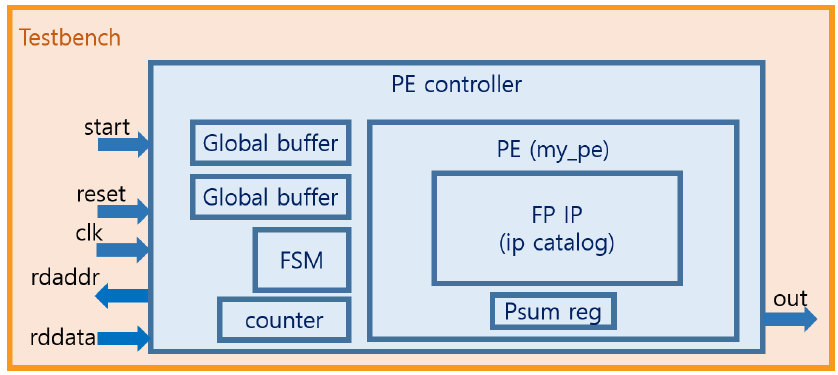
\includegraphics[width=0.6\textwidth]{fig/fig1.png}
\caption{PE와 FSM이 결합된 2개의 벡터의 내적을 연산하는 PE Controller module이다~\cite{lab6}.}
\label{fig1}
\end{figure}

\section{Implementation}
이번 프로젝트는 지난 프로젝트에서 구현한 Processing Element와 이를 실행을 시키기 위해 사용되었던 테스트벤치 코드를 결합한 새로운 모듈을 구현하는 것을 목적으로 한다. PE Control 모듈은 추후 구현할 Matrix-Matrix Multiplication을 수행하기 위해 존재하는 하위 모듈이다. 아래는 코드 구현과 함께 아이디어 및 기능에 대한 설명이 진행된다.

\subsection{PE Controller}
Figure~\ref{fig1}을 참고하면 Practice \#5에서 구현한 벡터의 내적을 계산할 수 있는 \texttt{my\_pe} 모듈과 그것을 구성하는 Floating-point fused multiplier IP catalog가 존재한다. PE controller에서는 내적을 연산할 벡터의 모음을 Global buffer에 저장한 뒤 PE에 전달, 연산을 수행하게 된다. 상기된 Sequential logic 모듈이 상황에 따라 어떤 기능을 수행할 지 다르게 명시해주어야 하기 때문에 State를 정의하여 FSM의 논리를 모두 구현해준다.\\

PE controller는 IDLE, LOAD, CALC, DONE이라는 총 4가지 state를 가진다. IDLE은 대기 상태를 의미하며 이 때 
\texttt{start} 신호가 입력되면 LOAD state로 전이된다. 이 상태에서는 \texttt{rdaddr} 주소를 Testbench에 전달하여 \texttt{rddata} 값을 하나씩 입력받아 Global buffer에 저장한다.\\

모든 LOAD 과정이 마치면 CALC 단계에서 FP IP catalog를 수행하게 된다. Global buffer에 저장된 16개의 실수 벡터 2개를 추출하여 Multiply-Accumulator를 이용해 내적 값을 구하게 된다. 연산이 모두 끝난 후 state는 DONE으로 넘어가게 되고 5 사이클의 Latency를 가지고 \texttt{done} signal과 함께 결과 값을 반환한다. 5 사이클 이후에는 다시 state를 IDLE 상태로 돌려 놓고 \texttt{start} 신호를 기다린다.\\

\begin{itemize*}
\item 아래에 첨부된 코드 중 3-30 라인은 PE controller의 변수 선언에 관한 내용이다.
\begin{itemize*}
\item \texttt{parameter}에 포함된 (1) \texttt{L\_RAM\_SIZE}는 입력되는 벡터의 크기를 표현하는 상수이고 (2) \texttt{BITWIDTH}는 연산을 하기 위한 실수 자료형의 크기를 나타낸다. 나머지 입력과 출력에 관한 Wire는 모두 Figure~\ref{fig1}에서 표기한 바와 같다. 
\item FSM과 관련된 변수는 현재 상태와 앞으로 업데이트해야하는 상태 변수 \texttt{present\_state}와 \texttt{next\_state}가 있고 그 외에 Counter가 있다. 상태를 나타내는 상수는 총 네 가지로 $0 \sim 3$의 값을 \texttt{S\_IDLE}, \texttt{S\_LOAD}, \texttt{S\_CALC}과 \texttt{S\_DONE}에 해당하도록 설정하였다.
\item 내장 모듈인 MY\_PE의 입출력 변수 \texttt{ain}, \texttt{bin}, \texttt{valid}, \texttt{dout}, \texttt{dvalid}를 함께 선언하고 지정시켜주어야 한다.
\end{itemize*}

\item 32-23 라인과 42-78 라인은 강의시간에 배운 FSM의 format을 그대로 차용하여 구현하였다. 초기 상태를 \texttt{reset} 신호와 함께 IDLE 상태로 초기화 한다. 현재 상태에서 어떤 조건이 중족되었을 때 다음 상태를 지정해주는 논리를 구현해준다.
\begin{itemize*}
\item IDLE 상태에서 \texttt{start} 신호가 들어올 경우 LOAD로 전환. (44 라인)
\item LOAD 상태에서 테스트 벤치에서 모든 데이터 (\texttt{cnt\_load} 갯수 만큼의 데이터)를 전달받아 연산에 쓰일 값들이 Global buffer에 전부 저장이 되었을 경우 CALC로 전환. (45 라인)
\item CALC 상태에서 내장 모듈 MY\_PE에서 2개의 벡터의 크기만큼의 연산을 모두 마쳤을 경우 (\texttt{cnt\_calc} 갯수 만큼의 Fused multiplication 수행) DONE로 전환. (46 라인)
\item DONE 상태에서 Latency 만큼 딜레이가 진행된 후에 (Clock이 \texttt{cnt\_done} 만큼 경과된 후) IDLE로 전환. (47 라인)
\end{itemize*}

\item 50-60라인은 각 상태에 위치했을 때 어떤 Counter를 활성화 시킬지 지정해주는 부분이다. 62-65라인에서는 현재 상태가 LOAD에 이르렀을 때 테스트벤치로 \texttt{rdaddr}을 전달해주고 해당하는 실수형 자료 \texttt{rddata}를 받아와 Global buffer에 저장한다.
\end{itemize*}


\subsubsection*{\texttt{MY\_PE\_CONTROLLER}}
\begin{lstlisting}[style={verilog-style}]
`timescale 1ns / 1ps
module my_pe_controller #(
    parameter L_RAM_SIZE = 6,
    parameter BITWIDTH = 32
)(
    input start,
    input reset,
    input clk,
    output [L_RAM_SIZE:0] rdaddr,
    input [BITWIDTH-1:0] rddata,
    output [BITWIDTH-1:0] out,
    output done
);
    parameter DONE_LATENCY = 5;
    parameter S_IDLE = 2'd0, S_LOAD = 2'd1, S_CALC = 2'd2, S_DONE = 2'd3;
    reg [1:0] present_state, next_state;
    
    reg [L_RAM_SIZE:0] cnt_load, cnt_calc;
    reg [2:0] cnt_done;
    reg rst_cnt_load, rst_cnt_calc, rst_cnt_done;
    
    reg [BITWIDTH-1:0] gb1[0:2**L_RAM_SIZE-1];
    reg [BITWIDTH-1:0] gb2[0:2**L_RAM_SIZE-1];
    
    reg [BITWIDTH-1:0] ain;
    reg [BITWIDTH-1:0] bin;
    reg valid = 0;
    
    wire [BITWIDTH-1:0] dout;
    wire dvalid;
    
    always @(posedge clk or posedge reset)
        if (reset) present_state <= S_IDLE; else present_state <= next_state;
        
    always @(posedge clk or posedge rst_cnt_load) 
        if (rst_cnt_load) cnt_load <= 0; else cnt_load <= cnt_load + 1;
    always @(posedge clk or posedge rst_cnt_calc) 
        if (rst_cnt_calc) cnt_calc <= 0;
    always @(posedge clk or posedge rst_cnt_done) 
        if (rst_cnt_done) cnt_done <= 0; else cnt_done <= cnt_done + 1;
    
    always @(*)
        case (present_state)
            S_IDLE: if (start)                              next_state = S_LOAD; else next_state = present_state;
            S_LOAD: if (cnt_load == 2**(L_RAM_SIZE+1)-1)    next_state = S_CALC; else next_state = present_state;
            S_CALC: if (cnt_calc == 2**L_RAM_SIZE)          next_state = S_DONE; else next_state = present_state;
            S_DONE: if (cnt_done == DONE_LATENCY-1)         next_state = S_IDLE; else next_state = present_state;
        endcase
    
    always @(*)
        case (present_state)
            S_LOAD: rst_cnt_load <= 0;
            S_CALC: rst_cnt_calc <= 0;
            S_DONE: rst_cnt_done <= 0;
            default: begin
                rst_cnt_load <= 1; 
                rst_cnt_calc <= 1;
                rst_cnt_done <= 1;
            end
        endcase
        
    always @(rddata or present_state)
        if (present_state == S_LOAD) begin
            if (cnt_load < 2**L_RAM_SIZE) gb1[cnt_load] = rddata; else gb2[cnt_load-2**L_RAM_SIZE] = rddata;
        end
    
    always @(dvalid or present_state)
        if (present_state == S_CALC) begin
            if (dvalid) begin
                cnt_calc <= cnt_calc + 1;
                valid <= 0;
            end
            else begin
                ain <= gb1[cnt_calc];
                bin <= gb2[cnt_calc];
                valid <= 1;
            end
        end
    
    assign rdaddr = present_state == S_LOAD ? cnt_load : 0;
    assign out = present_state == S_DONE ? dout : 0;
    assign done = present_state == S_DONE ? 1 : 0;
    
    my_pe #(L_RAM_SIZE, BITWIDTH) MY_PE(
        .aclk(clk),
        .aresetn(~reset),
        .ain(ain),
        .bin(bin),
        .valid(valid),
        .dvalid(dvalid),
        .dout(dout)
    );
endmodule
\end{lstlisting}

코드의 하단부에는 지난 실습에서 구현한 Floating point MAC모듈의 호출 부분이다. Parameter에 들어가는 값은 모두 변수명과 동일하게 매칭을 해주었다~\cite{lab5, thomas2008verilog}.

\newpage
\section{Result}

\subsection{Testbench Implementation}
\label{sec:testbench}
아래의 코드는 MY\_PE\_CONTROLLER의 구현의 Validity를 확인하기 위해 검증 시나리오를 설정하고 그에 맞게 구현한 것이다. MY\_PE\_CONTROLLER 인스턴스를 입력 벡터의 크기, $2^\texttt{L\_RAM\_SIZE}= 2^4=16$와 저장되는 실수의 자료형 크기, $\texttt{BITWIDTH}=32$를 사용하여 선언하였다.\\
전체적인 testbench의 수행순서는 다음과 같다. 1. 두 개의 벡터 데이터의 초기화 및 설정. 2. floating\_point\_MAC의 정상적인 동작을 위한 기본설정. 3. MY\_PE\_CONTROLLER의 동작 과정에서 data load요청이 들어왔을 때, 요청한 주솟값의 데이터 전달.\\

아래는 작성된 코드의 자세한 설명이다.
\begin{itemize*}
\item 내적 연산을 위해서는 두 개의 벡터가 필요하고, 하나의 벡터당 크기가 16이므로, 총 32개의 데이터가 초기화되는 셈이다. 따라서, 먼저 \texttt{gb1}(첫번째 벡터), \texttt{gb2}(두번째 벡터)의 값들을 초기화 시켜주었다. 초기화된 데이터의 전체 주소는 0x00-0x1f 이고, \texttt{gb1}가 0x00-0x0f, \texttt{gb2}가 0x10-0x1f의 주소를 갖는다 (16-19 라인).\\

\item testbench에서 가장 먼저 수행한 작업은 floating\_point\_MAC을 초기화한 것이다. reset 값을 1로 설정한 후, 적절한 clock cycle만큼 기다려주었다. 그 이후, start 값을 1로, reset 값을 0으로 설정하여 MY\_PE\_CONTROLLER 가 동작하도록 하였다 (21-26 라인).\\

\item \texttt{always} 구문을 사용하여, rdaddr(주솟값의 데이터 요청)이 들어왔을 때, 해당 주소의  벡터 데이터를 제공해준다 (30-31 라인).
\end{itemize*}

\subsubsection*{\texttt{TB\_MY\_PE\_CONTROLLER}}
\begin{lstlisting}[style={verilog-style}]
`timescale 1ns / 1ps
module tb_my_pe_controller #(
    parameter L_RAM_SIZE = 4,
    parameter BITWIDTH = 32
)();
    reg [BITWIDTH-1:0] gb[0:2**(L_RAM_SIZE+1)-1];
    reg [BITWIDTH-1:0] rddata;
    wire [BITWIDTH-1:0] out;
    wire [L_RAM_SIZE:0] rdaddr;
    wire done;
    
    reg start, clk, reset;
    integer i;
    
    initial begin
        for(i = 0; i < 2**L_RAM_SIZE; i = i+1) begin
            gb[i]                 = $urandom_range(2**30, 2**30+2**24);
            gb[2**L_RAM_SIZE + i] = $urandom_range(2**30, 2**30+2**24);
        end
    
        clk <= 0;
        start <= 0;
        reset <= 1; #20;
        
        start <= 1;
        reset <= 0; #20;
    end
    
    always #5 clk = ~clk;
    always @(rdaddr) begin
        rddata = gb[rdaddr];
    end
    
    my_pe_controller #(L_RAM_SIZE, BITWIDTH) MY_PE_CONTROLLER(
        .start(start),
        .reset(reset),
        .clk(clk),
        .rdaddr(rdaddr),
        .rddata(rddata),
        .out(out),
        .done(done)
    );
endmodule
\end{lstlisting}

\subsection{Simulation Results}
Section~\ref{sec:testbench}에서 구현된 테스트 벤치를 실행하면 아래 Figure~\ref{fig2}와 같은 Waveform을 확인할 수 있다. 결과를 자세히 보면, \texttt{start}가 high일 때 MY\_PE\_CONTROLLER가 동작을 시작하고, LOAD\_STATE일 때, 주솟값을 요청하여 데이터를 받고, CALC\_STATE일 때, floating\_point\_MAC의 동작으로 출력값을 계산하는 것을 볼 수 있다. 모든 계산이 완료되면, \texttt{done}이 high가 되며, 최종 결과값을 \texttt{out}으로 출력한다.\\

아래의 Table~\ref{tab1}은 \texttt{TB\_MY\_PE\_CONTROLLER} 17-18 라인에서 생성된 테스트 데이터이며 벡터 \texttt{ain}과 \texttt{bin}의 내적 결과값을 구하기 위해 각 원소별로 곱셈 결과값을 3열에 연산하였고 이를 누적하여 마지막에 약 323.0319 라는 결과값을 가지는 것을 확인할 수 있다. 아래의 Figure~\ref{fig3}의 \texttt{CALC} 상태와 \texttt{DONE} Waveform을 확인하면 같은 값이 출력됨을 알 수 있다.

\begin{table}[htb]
\renewcommand*{\arraystretch}{1.4}
\begin{center}
\begin{tabular}{ |c|c|c|c| } 
 \hline
 \textbf{\texttt{index}} & \textbf{\texttt{ain}} & \textbf{\texttt{bin}} & \textbf{\texttt{dout}} \\ 
 \hline
1 & 7.80244779586791 & 5.81660604476929 & 45.3837650134422 \\
2 & 4.89655828475952 & 4.23463726043701 & 66.1189131739864 \\
3 & 3.40448760986328 & 2.32309341430664 & 74.0278559195483 \\
4 & 2.79091644287109 & 3.30574178695679 & 83.2539050286521 \\
5 & 6.46279287338257 & 6.47845220565796 & 125.122799773928 \\
6 & 6.84624338150024 & 2.63594484329224 & 143.169119711317 \\
7 & 7.12470054626465 & 2.21409893035889 & 158.943911569929 \\
8 & 3.94174790382385 & 5.58761501312256 & 180.96888133528 \\
9 & 6.90677261352539 & 3.36496090888977 & 204.209901186383 \\
10 & 6.85968828201294 & 6.03147268295288 & 245.583923672916 \\
11 & 3.57905983924866 & 3.37159180641174 & 257.651052501584 \\
12 & 3.80960464477539 & 3.03244590759277 & 269.20347251618 \\
13 & 5.47310543060303 & 3.23944854736328 & 286.933315952913 \\
14 & 2.04824304580688 & 2.31567335128784 & 291.676377791048 \\
15 & 5.22220277786255 & 3.8579089641571 & 311.82316070041 \\
16 & 3.34818053245544 & 3.34771490097046 & 323.031914560051 \\
\hline
\end{tabular}
\caption{Testbench dataset}
\label{tab1}
\end{center}
\end{table}

\begin{figure}[htb!]
	\centering
	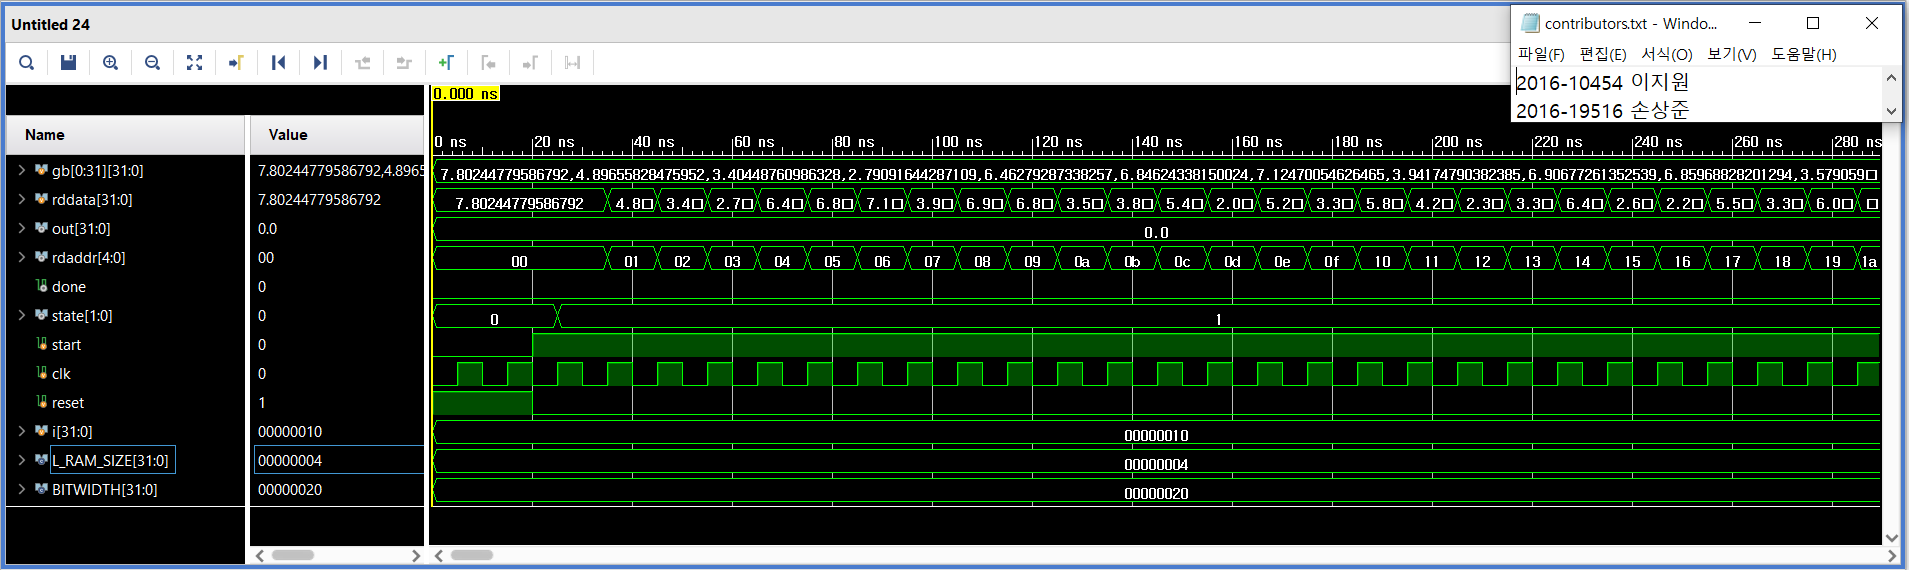
\includegraphics[width=1.0\textwidth]{fig/My_PE_Controller_Waveform1.png}
	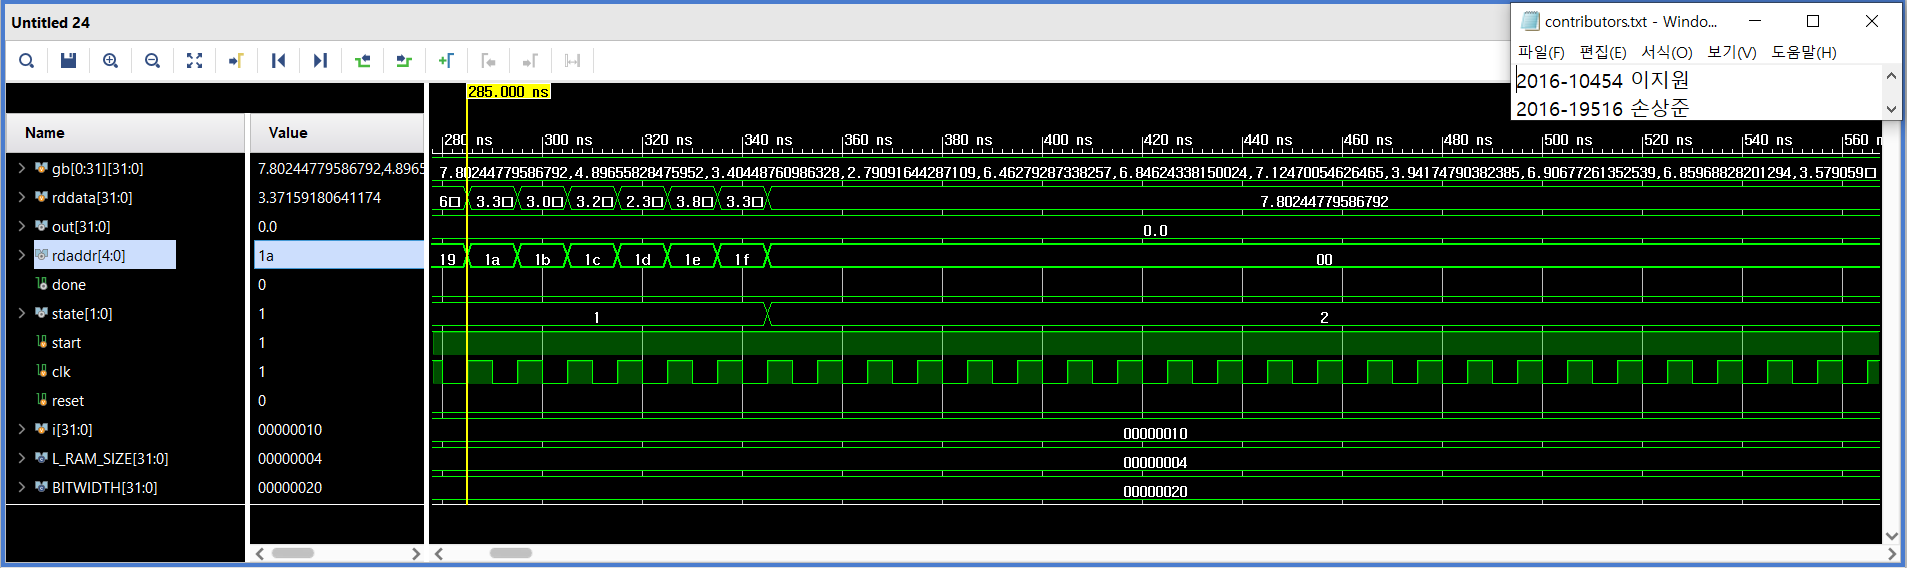
\includegraphics[width=1.0\textwidth]{fig/My_PE_Controller_Waveform2.png}
	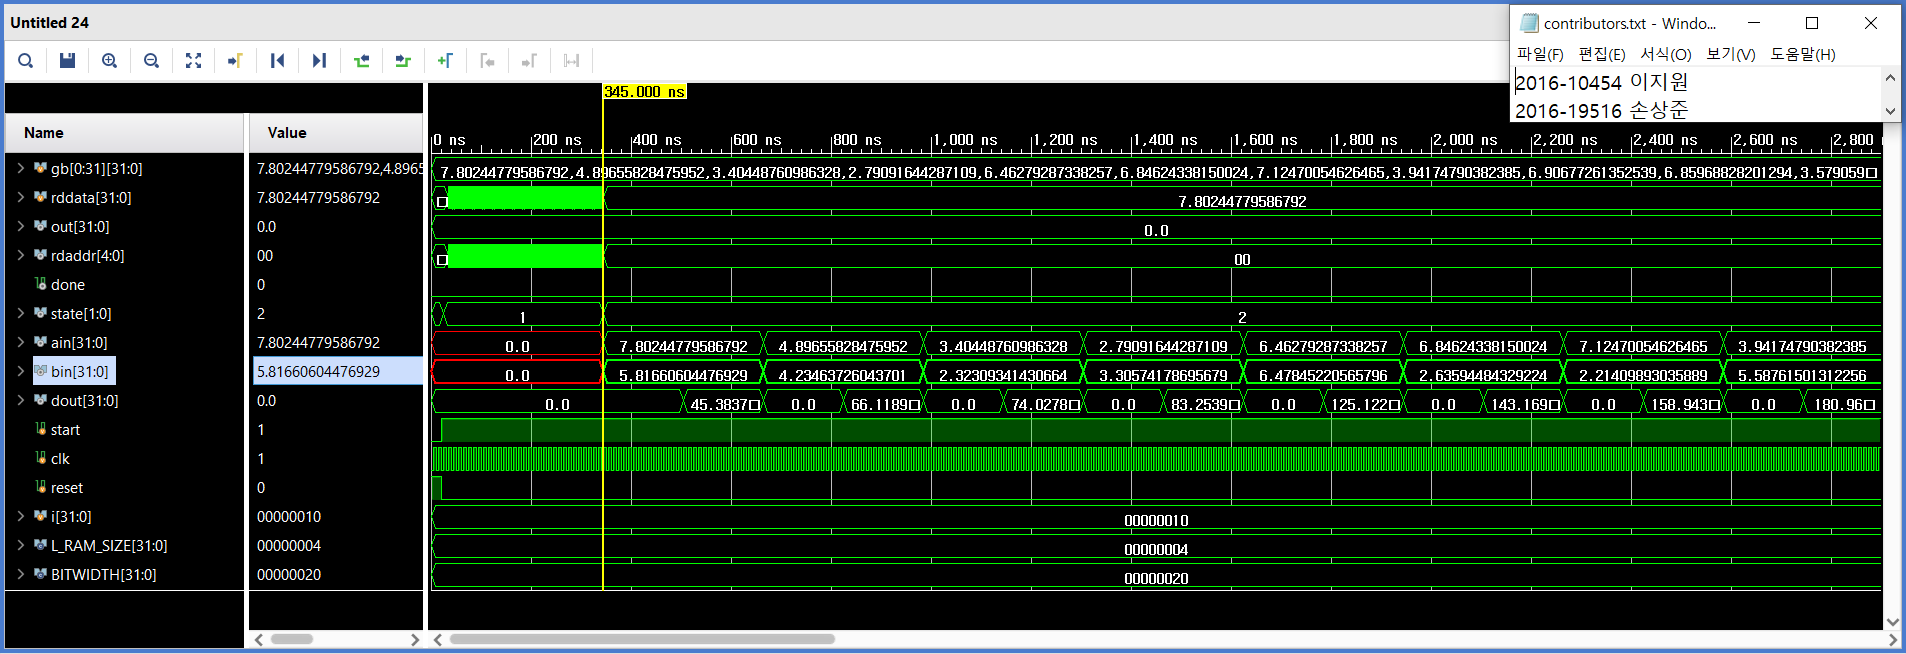
\includegraphics[width=1.0\textwidth]{fig/My_PE_Controller_Waveform3.png}
\caption{\texttt{IDLE}, \texttt{LOAD}, \texttt{CALC} 전환이 되는 동안의 Waveform이다. 중간에 \texttt{state}를 출력하여 Controller 모듈의 FSM이 제대로 된 기능을 하는지 볼 수 있다. 또한 \texttt{CALC}에서 하위 모듈 \texttt{MY\_PE}에 올바른 입력과 출력이 이뤄지는지 확인을 위해 \texttt{ain}, \texttt{bin}, \texttt{dout}을 함께 비교하였다.}
\label{fig2}
\end{figure}


\begin{figure}[htb!]
	\centering
	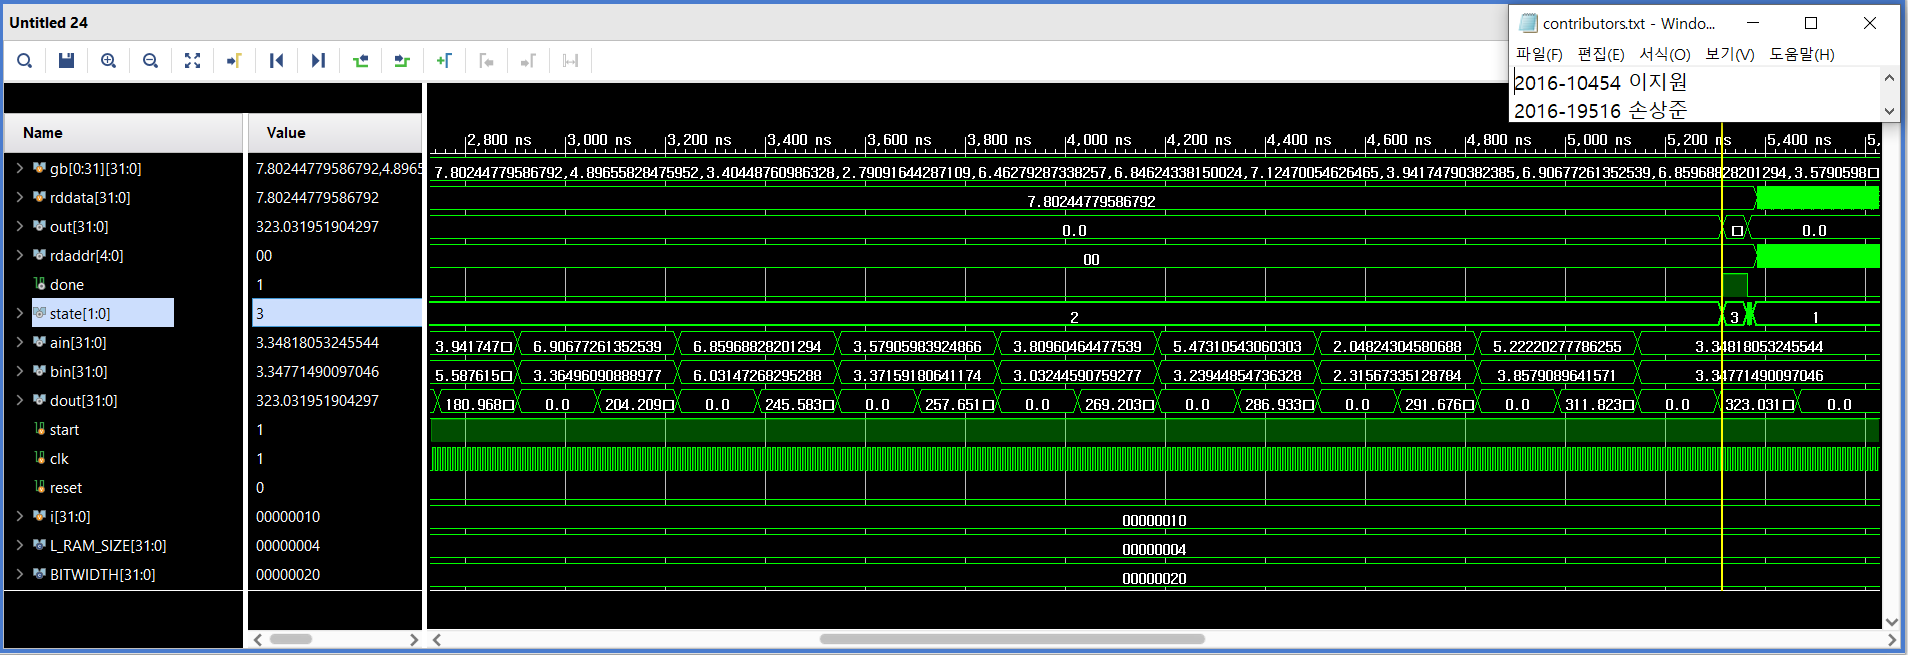
\includegraphics[width=1.0\textwidth]{fig/My_PE_Controller_Waveform4.png}
	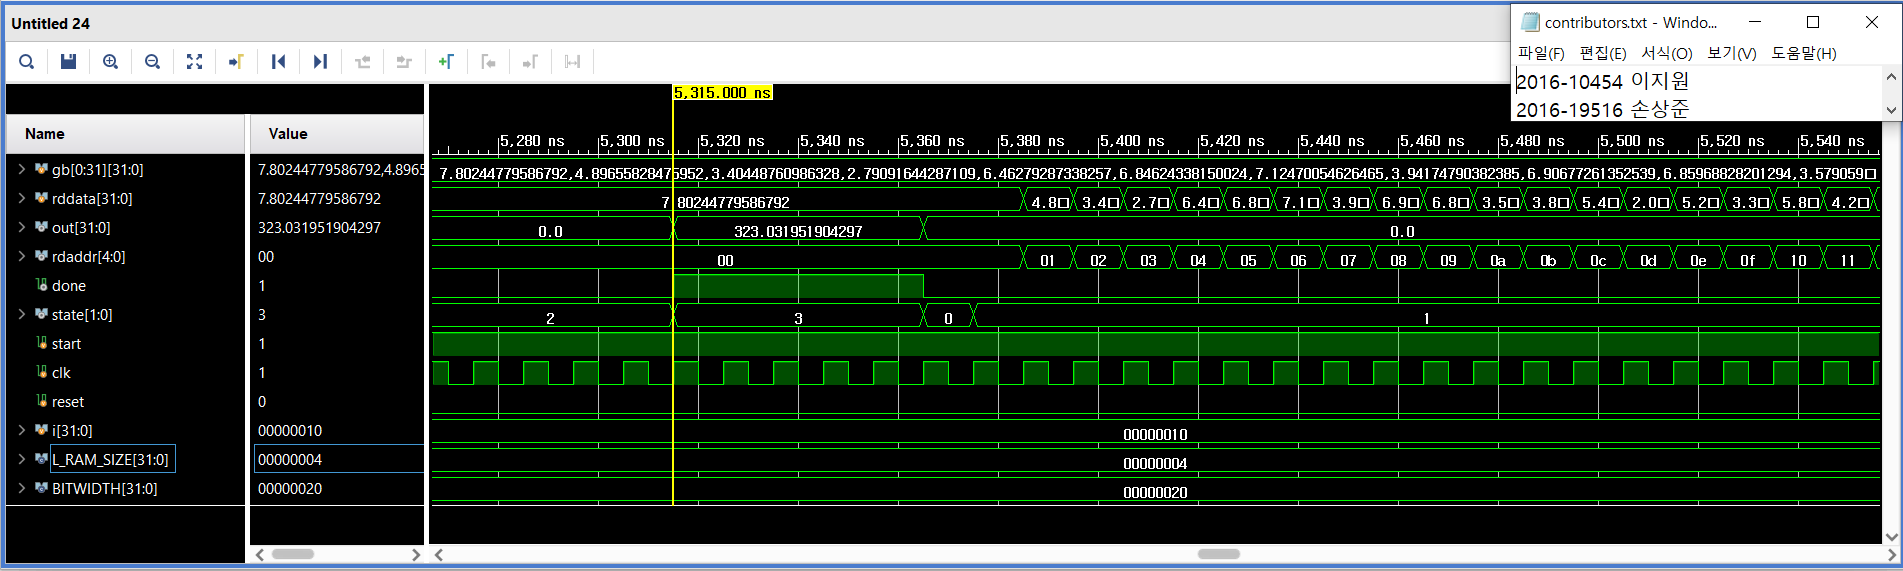
\includegraphics[width=1.0\textwidth]{fig/My_PE_Controller_Waveform5.png}
\caption{\texttt{CALC}, \texttt{DONE}, 다음 \texttt{IDLE} 전환이 되는 동안의 Waveform이다. 벡터 내적 결과값이 \texttt{out}에 \texttt{done} 신호와 함께 5 Cycle 동안 지속되고 \texttt{start} 신호가 활성화 되어 같은 작업을 기존 \texttt{out}에 누적하여 연산을 반복하는 것을 볼 수 있다.}
\label{fig3}
\end{figure}

\newpage
\subsection{Design Implementation}
Figure~\ref{fig4}는 구현된 MY\_PE\_CONTROLLER를 synthesis, implementation을 하였을 때 나오는 implementation design 결과이다.

\begin{figure}[htb!]
	\centering
	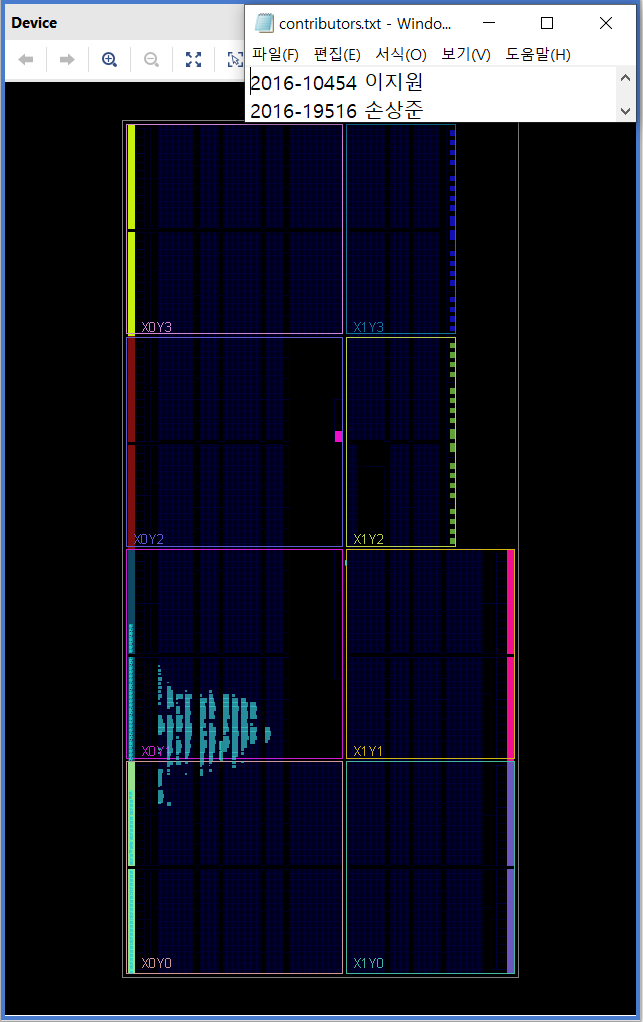
\includegraphics[width=0.49\textwidth]{fig/My_PE_Controller_Design1.png}
	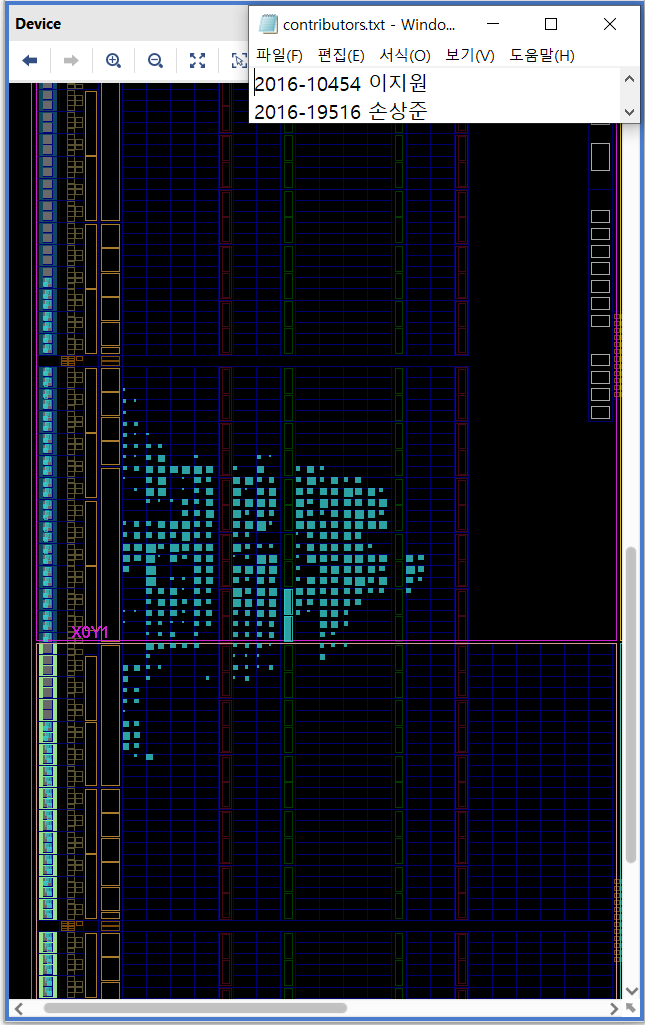
\includegraphics[width=0.49\textwidth]{fig/My_PE_Controller_Design2.png}
\caption{Implementation design, \texttt{MY\_PE\_CONTROLLER} 모듈을 Synthesis와 Implementation을 진행하고 보드에 어느 부분을 사용하는 지 시각화 시킨 것이다. 좌측에 전반적인 보드와 특히 많이 사용된 \texttt{X0Y1}를 확대한 결과이다.}
\label{fig4}
\end{figure}

\newpage
\section{Conclusion}
이번 과제는 고려해야 할 것들이 많았다. counter를 이용하여 LOAD 데이터 갯수 설정, floating\_point\_MAC의 계산 횟수, DONE\_STATE에서의 latency 설정을 제어해 주었다.\\

CALC\_STATE에서 latency에 관계없이 올바른 결과값이 출력되도록 하는 부분의 구현이 까다로웠는데, 먼저 MY\_PE에서 dvalid값을 clk에 동기화 시켜주었다. 이후에, MY\_PE\_CONTROLLER에서 dvalid가 high이고, 모든 계산을 마쳤을 때 state를 바꿔줌으로써 done state일 때 올바른 결과값을 출력해내었다.\\

이번 과제를 수행하면서 올바른 시뮬레이션 결과를 얻었지만, synthesis와 implementation이 정상적으로 되지 않는 경우가 있었다. 이를 고쳐나가면서, 어느 구문들이 implementation이 되지 않는지, net이 동시에 업데이트 되어 충돌되는 부분은 없는지 등을 확인하며 구현해야겠다고 생각하였다.\\

\bibliographystyle{plain}
\bibliography{other}

\end{document}
